\documentclass{article}[11pt]
\textheight 8.5in
\usepackage{graphicx}
\usepackage{float}%for forcing position of figs
\usepackage{hyperref}
\usepackage{amsmath}
\usepackage{amssymb}

\begin{document}
\begin{center}
Siddharthan Rajasekaran\\
Week of 3/13/2017 - 3/20/2017
\end{center}

\section{Summary of Discussions}
In this report, we will talk about the initial implementation of Maximum entropy IRL. We will also discuss about the limitations and why we need to learn non-linear reward functions. 

\section{Grid world}
We pick the same grid world given in SVM based IRL paper to implement a proof of concept. The grid has a dimension of $128 \times 128$ (2-D). This grid is further divided into macro cells of $16 \times 16$ grid cells. Hence there are $8\times8$ = 64 macro cells. Each cell is initialized with a random reward from $[-1,1]$. These reward values are stored in the weight vector $w$. The dimension of this weight vector is $(64\times 1)$. We have a indicator feature vector $\phi(x,y)$ which is again $(64\times 1)$ and $i^{th}$ dimension of it is $1$ if $(x,y)$ belongs to $i^{th}$ macro cell and $0$ otherwise. Using the weight and the feature vectors, the reward function can be written as $$R(x,y) = w^T\phi(x,y)$$ According to the constraints in the algorithm that the total reward can never exceed $1$, we normalize $w$ using $w := \frac{w}{||w||_1}$. Given this reward function (for any $w$) we can compute the optimal action under the reward using value iteration \cite{russell1995modern} which can be used as demonstrations for IRL.


\section{Method}
In MaxEnt IRL we solve the problem of maximizing the causal entropy subject to meeting the feature expectation of the demonstrations. The problem is given in Ziebart's thesis \cite{ziebart2010modeling} (page 72 Eq. 6.1. The solution to the maximum entropy problem is often of the form $\frac{\exp(\lambda_1f_1(x))}{Z(\lambda_1)}$ if the expectation of the function $f_1(x)$ under the probability distribution is given by some $F_1$ (in fact this is the constraint used to identify $\lambda_1$). For this problem, since the causal entropy involves a series of products, we can express the solution through a recursive update (Eq. 6.2 in \cite{ziebart2010modeling}). The partition functions $Z_{S_{1:t}, A_{1:t-1}, w}$ in this update , is the complete exponential reward mass at state $S_t$. For instance, at $t=T$, the terminal time, $Z_{S_{1:T}, A_{1:T-1}, w} = \exp(w^T\mathcal{F}(\textbf{S}, \textbf{A}))$. Here, $w^T\mathcal{F}(\textbf{S}, \textbf{A})$ is cumulative reward that the expert achieved. In the maximum entropy solution since the reward appears in the exponents, it can be seen that the complete reward is in fact achieved at the end of $T^{th}$ time step. $Z_{A_t|S_{1:t}, A_{1:t-1}, w}$ is the mass of exponentiated reward that should be propagated backwards to $S_t$ from $S_{t+1}$ through action $A_{t}$. This way we can recursively perform a backward pass until all the exponentiated reward mass has been distributed among the possible paths according to the maximum entropy principle (probability of a path is proportional to the exponentiated cumulative reward collected under that path).  

Interesting thing here to note is that (as pointed out in \cite{ziebart2010modeling}) the $\log$ of the actions and state partitions can be interpreted as Q-value and Value function of MDP under soft-Bellamn equations. \cite{asadi2016new} introduces a new softmax operator, mellowmax,  to form soft-Bellman equations. 

\begin{align}
mm_\omega(\textbf{X}) = \frac{\log( \frac{1}{n} \sum_{i=1}^n e^{\omega x_i})}{\omega}
\end{align}
However, the solution to maximum entropy problem (Eq. 6.1 in Ziebart's thesis \cite{ziebart2010modeling}) has two difference from the above millowmax operator. There is no parameter $\omega$ and $\frac{1}{n}$. However, the essential properties of softmax operator (as enumerated in \cite{asadi2016new}) for the value iteration to converge to the optimal values (unique values) is met even without $\frac{1}{n}$ (we can just set $\omega =1$ to remove it). The value of the parameter $\omega$ corresponds to how random the policy will be. Higher the value of $\omega$ the more deterministic the policy will be and the solution will be exploiting and not exploring $lim_{\omega \to \infty} mm_\omega = max$. 

The softmax operator in maximum entropy is thus defined as
\begin{align*}
softmax_x f(x) \triangleq log \sum_x e^{f(x)}
\end{align*}
Hence the value iteration problem (using log of partitions) becomes

\begin{align}
  Q^{soft}_{k+1}(s_t,a_t) &\triangleq \log Z_{a_t|s_t} = R(s_t) + \gamma\sum_{s_{t+1}} P(s_{t+1}|s_t,a_t)V^{soft}_k(s_{t+1})\\
  V_{k+1} &\triangleq \log Z_{s_t} = softmax_{a_t} \ Q^{soft}_{k+1}(s_t,a_t)
\end{align} 
Note that this is regular Bellman equations where the max operator is replaced with softmax. WE have introduced the discount factor $\gamma$ which is not in Algorithm 9.1 in Ziebart's thesis. This is a necessary requirement for extending the method to infinite horizon problems with no terminal states\cite{bloem2014infinite}. However, \cite{bloem2014infinite} introduces a entropy discounting factor $\beta$ which still has to be included in our implementation. If we take the case of $\beta = \gamma$, \cite{bloem2014infinite} reduces exactly to our implementation. 

The policy under the above formulation is given by 

\begin{align}
\pi(a_t|s_t) =  \frac{Z_{a_t|s_t}}{Z_{s_t}} = e^{Q^{soft}(a_t|s_t) - V^{soft}(s_t)}
\end{align}

\textbf{Implementation note}: Since we are taking log of exponents of large numbers during value iteration and taking exponents of logs to revert the policy back, the policy is not normalized over action. So we just use linear normalization to make sure $\sum_{a_t} \pi(a_t|s_t) = 1$. 

Once we have the policy, one can compute the state visitation frequencies using the MDP model. This is analogous to motion update in POMDPs. For this we use the forward pass Algorithm in Ziebart et. al \cite{ziebart2008maximum}. \textbf{The Algorithm 9.3 in Ziebart's thesis \cite{ziebart2010modeling} does not look right but we should confirm this again}. Given the initial distribution of the agent, we propagate the probability mass according to the stochastic policy and the transition dynamics of the MDP. 

\begin{align}
\label{eq:pomdp}
&bel_{t=0} = P(s_i = s_{initial}) 
\end{align} 
\begin{align*} 
&\textbf{for N steps:} \\
&bel_{t+1} = \sum_{a_t}\sum_{s_z}bel_t(s_t)\pi(a_t|s_t)P(s_z|s_t,a_t) \\
&\textbf{End for} \\
&D_{s_i} = \sum_t \gamma^t bel_t \ \ \ \forall s_i
\end{align*} 
In the above algorithm, we have introduced $\gamma^t$ to discount for the infinite horizon case. In \cite{ziebart2008maximum}, it is unclear what value of $N$ should be chosen. However, it is actually the length of the demonstration. This is because, if we compute the state visitation frequencies (and thus the feature expectation) for longer time than the length of the demonstration, we might want to stay longer in the absorbing state at the end of out policy. This results in higher state visitation at absorbing states than that in the demonstration. 

\textbf{Implementation note}: One has to make sure that the feature expectation under the demonstration is the same as that computed using the POMDP prediction step \ref{eq:pomdp} with the policy followed during the demonstration in case of deterministic MDP. Otherwise, it means that for the same demonstration, a rollout will result in a different state visitations than using our algorithm above.

 
\section{Results of implementation}

The value iteration is of the order $\mathcal{O}(|\mathcal{S}||\mathcal{A}||\mathcal{T}||\mathcal{I}|)$ where $|\mathcal{T}|$ the possible number of states that we can land after taking an action and $|\mathcal{I}|$ is the number of iterations to converge which is $poly(|\mathcal{S}|,|\mathcal{A}|, \frac{1}{1-\gamma})$. In case of normal value iteration (as opposed to the soft version), where we can get deterministic policy, it is possible to do policy iteration which converges faster than the value iteration. Since we have continuous probabilities defining policy, we have to iterate till the value iteration converges. This takes more time than policy iteration. However, the main reason for the algorithm being slow is that  SVM-IRL takes about 5 iteration on an average to converge. In case of MaxEnt IRL, we run the gradient descent with a learning factor of $0.01$ for $200$ epochs. This takes huge amounts of time. 

Note: Can we use optimizers to solve the problem faster?. The paper says the problem is convex in deterministic setting. Can we figure out a way to use optimizers this to non-deterministic cases?. Also, Ziebart's thesis has some ways to approximate the maximum entropy (using state ordering) algorithm to get better computation times. We can implement the approximate algorithm in case we employ MaxEnt IRL on human arm (higher DoF).  

In the figure below, we have a $5\times5$ grid with a positive reward (+1) at $(5,5)$ and 0 elsewhere. We take 20 demonstrations all starting at $(0,0)$ with a policy that takes `North' and `East' with equal probabilities (0.5 and 0.5 respectively). Of the 20 demonstration most of them ($14$) make it to the goal while other get stuck at the right or the top walls. Note that the recovered reward wants to best explain the actions assuming that the expert acted to maximize entropy. This can be seen as a gradual change in the shading from blue (in the bottom left) to red (in the top right). Also the right and the top edge have more reward than their neighbors since some of the demonstrations get stuck at these places. 
 


\begin{figure}[H]
  \begin{center}
    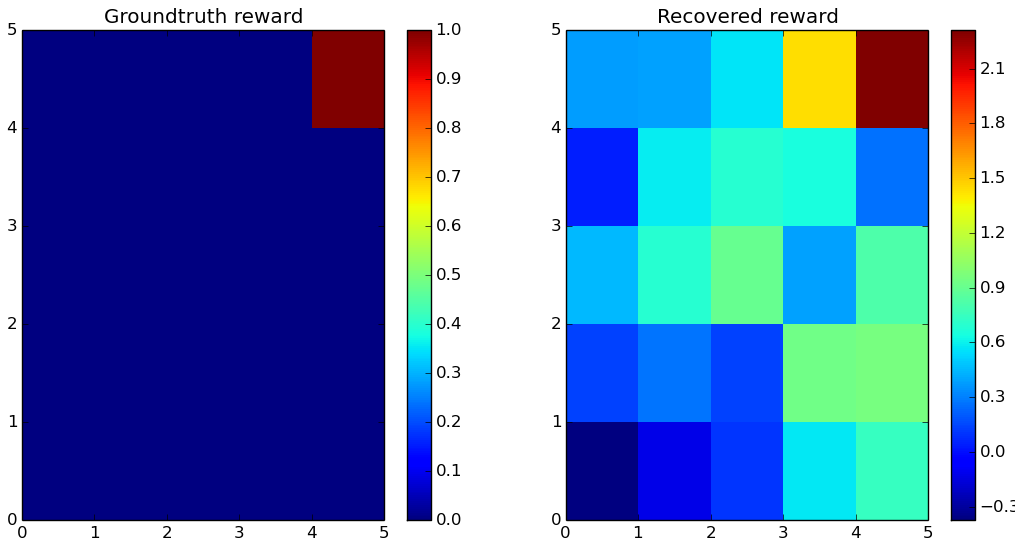
\includegraphics[width=1\linewidth]{images/max_entresults}
    \caption{Recovering the reward function using demonstrations using MaxEnt IRL. On the left is the ground truth and on the right is the recovered reward. Note how the recovered reward has higher magnitudes to reason about the preference of actions in demonstration}
    \label{fig:converge}
  \end{center}
\end{figure}



\section{Problems with linear reward}

Though the MaxEnt solution alleviates the problem when there can be multiple behaviors with the same reward (by choosing all behaviors equally likely) and also finds a weight that explains behavior of the expert which will other wise be sub-optimal in normal RL setting (with max operator), it does not solve the problem of the actual reward function not being able to be represented as linear sum over the features. This can be solved using two approaches: 1) Adaptive features or learning the features \cite{dvijotham2010inverse, levine2010feature} and 2) Using the kernel trick - GPIRL \cite{levine2011nonlinear}. GPIRL looks promising since it also incorporates MaxEnt IRL but only chooses to represent the reward as a Gaussian Process. 

GPIRL formulates the IRL problem as GP regression problem (maximizing the posterior - probability of parameters given the demonstration). THe method specifies the kernel function used (ARD - kernel) and makes some sparsifying assumptions on the GP regression problem using inducing points \cite{quinonero2005unifying} for more efficient calculations. The results of the method looks very promising since it actually finds the non linear reward under which the human is actually optimal. Also, since we do not specify the feature mapping, the kernel function translates to an infinite dimensional feature which can capture the unique behavior of the expert (In other words, GPs allow humans to be optimal under some nonlinear reward function). 




\section{Plan for next week}
I am planning to implement the GPIRL algorithm and test it on the same grid world problem to compare it to other problems. I would like to clearly understand the relation between Linearly solvable MDPs and MaxEnt IRL. 

\section{Long-Term Plan}
Once we have these algorithms working, I would like to focus on finding problems with them that make it hard for us to extend to predicting human actions reliably (which as I understand is a problem in itself!). 

One of such problems is to get the discount factor $\gamma$ from the demonstration (as suggested by Prof. Fu). In the SVM-IRL implementation, with (small values) $\gamma = 0.9$, the learned behavior did not imitate the expert after 20 time steps as any behavior would hardly affect the feature expectations (as they are heavily discounted in later time steps). Taking $\gamma = 0.99$, we see the algorithm struggling to converge if the demonstrations were taken with optimal policy corresponding to  $\gamma = 0.9$. This is because, the expert is very myopic and does not want to cross 0 reward regions to reach a state with very high reward (since it would be discounted by then). But assigning any $w$ with $\gamma = 0.99$ does not give raise to this behavior and we need to mix many policies to get there. In case of MaxEnt IRL, with $\gamma = 0.99$ we get non-zero gradients in large state spaces (128x128). However, with $\gamma = 0.9$, the gradient is almost zero since any behavior get penalized very less in most places since such behavior will only get lesser or negative rewards in later time-steps. 

Another interesting problem (as suggested by Prof. Li) is to incorporate linear reward feature in GP by deriving a kernel function that captures those linear rewards. However, the kernel function is a transformation of input space to a continuous infinite dimensional feature space. Understanding this mapping will be necessary for us to incoporate known features in the kernel


\section{Backlogs in MaxEnt IRL}
As we can see, the Maximum Entropy solution is very closely related to Linearly solvable MDPs. I tried to derive the maximum entropy equations for policy from the power method used in \cite{dvijotham2010inverse} to find the largest Eigen vector (which is the solution to the MDP). However, they do not seem to relate directly to the partitions given in the backward pass in \cite{ziebart2008maximum}. Fortunately, \cite{dvijotham2010inverse} gives a solution to IRL using Linearly solvable MDPs and explains how MaxEnt solution is related to \cite{dvijotham2010inverse}. Also, complete understanding of \cite{bloem2014infinite} will let me summarize MaxEnt IRL as a whole. 

\section{Bibliography}

\bibliographystyle{plain}
\bibliography{bibfile}
\end{document}
